\documentclass[polish,polish,a4paper]{article}
\usepackage[polish]{babel}
\usepackage[T1]{fontenc}
\usepackage[utf8]{inputenc}
\usepackage{pslatex}
\usepackage{pgfplots}
\usepackage{circuitikz} 
\usepackage{setspace}
\usepackage{caption}
\usepackage{amssymb}
\usepackage{amsmath}
%\usetikzlibrary{circuits.ee.IEC}
\usepackage{anysize}
\usepackage{graphicx}
\usepackage{hyperref}
\usepackage{float}
\hypersetup{
	colorlinks=true,
	linkcolor=blue,
	filecolor=magenta,      
	urlcolor=cyan,
}
\urlstyle{same}

\marginsize{2.5cm}{2.5cm}{2cm}{2cm}

\newcommand{\PRzFieldDsc}[1]{\sffamily\bfseries\scriptsize #1}
\newcommand{\PRzFieldCnt}[1]{\textit{#1}}
\newcommand{\PRzHeading}[8]{
	%% #1 - nazwa laboratorium
	%% #2 - kierunek 
	%% #3 - specjalność 
	%% #4 - rok studiów 
	%% #5 - symbol grupy lab.
	%% #6 - temat 
	%% #7 - numer lab.
	%% #8 - skład grupy ćwiczeniowej
	
	\begin{center}
		\begin{tabular}{ p{0.32\textwidth} p{0.15\textwidth} p{0.15\textwidth} p{0.12\textwidth} p{0.12\textwidth} }
			
			&   &   &   &   \\
			\hline
			\multicolumn{5}{|c|}{}\\[-1ex]
			\multicolumn{5}{|c|}{{\LARGE #1}}\\
			\multicolumn{5}{|c|}{}\\[-1ex]
			
			\hline
			\multicolumn{1}{|l|}{\PRzFieldDsc{Kierunek}}	& \multicolumn{1}{|l|}{\PRzFieldDsc{Specjalność}}	& \multicolumn{1}{|l|}{\PRzFieldDsc{Rok studiów}}	& \multicolumn{2}{|l|}{\PRzFieldDsc{Symbol grupy lab.}} \\
			\multicolumn{1}{|c|}{\PRzFieldCnt{#2}}		& \multicolumn{1}{|c|}{\PRzFieldCnt{#3}}		& \multicolumn{1}{|c|}{\PRzFieldCnt{#4}}		& \multicolumn{2}{|c|}{\PRzFieldCnt{#5}} \\
			
			\hline
			\multicolumn{4}{|l|}{\PRzFieldDsc{Temat Laboratorium}}		& \multicolumn{1}{|l|}{\PRzFieldDsc{Numer lab.}} \\
			\multicolumn{4}{|c|}{\PRzFieldCnt{#6}}				& \multicolumn{1}{|c|}{\PRzFieldCnt{#7}} \\
			
			\hline
			\multicolumn{5}{|l|}{\PRzFieldDsc{Skład grupy ćwiczeniowej oraz numery indeksów}}\\
			\multicolumn{5}{|c|}{\PRzFieldCnt{#8}}\\
			
			\hline
			\multicolumn{3}{|l|}{\PRzFieldDsc{Uwagi}}	& \multicolumn{2}{|l|}{\PRzFieldDsc{Ocena}} \\
			\multicolumn{3}{|c|}{\PRzFieldCnt{\ }}		& \multicolumn{2}{|c|}{\PRzFieldCnt{\ }} \\
			
			\hline
		\end{tabular}
	\end{center}
}



\begin{document}
	
	\PRzHeading{Laboratorium Podstaw Elektroniki}{Informatyka}{--}{I}{I3}{Ćwiczenia wprowadzające}{1}{Piotr Więtczak(132339), Robert Ciemny(136693), Kamil Basiukajc(136681)}
	
	
	\section{Ćwiczenia wprowadające}
	\subsection{Rezystory}
	
	\subsubsection*{Cel}
	
	W tym ćwiczeniu należy odczytać wartość rezystancji na podstawie kodu paskowego rezystorów lub oznaczeń
	oraz dokonać pomiaru wartości rezystancji przy pomocy multimetru RIGOL DM3051, pamiętając przy tym o
	poprawnym zapisaniu jednostek podczas wypełniania tabeli \hyperref[eq:tab1]{1}.
	
	\begin{spacing}{1,5}
		
		\subsubsection*{Wartości odczytów i wyniki pomiarów rezystancji }
		
		
		\begin{equation*}
		\label{eq:tab1}
		\begin{array}{|c|c|c|c|}
		\hline
		R&Barwa/oznaczenia&Odczyt&Pomiar \\ 
		\hline
		R_{1}&$  żółty - fioletowy - czewony - złoty  $ &4.7k \Omega& 4.634 k \Omega  \\ 
		\hline
		R_{2}&$ czerwony - czarny - zielony - złoty $ &2M \Omega& 2.009 M \Omega  \\ 
		\hline
		R_{3}&$ czerwony - czerwony - czerwony - złoty $&2.2k \Omega& 2.132k \Omega  \\ 
		\hline
		R_{4}&$ czerwony - czerwony - brązowy - złoty  $&220 \Omega&219.320 \Omega \\ 
		\hline
		R_{5}&$ brązowy - czarny - czerwony - złoty $&1k \Omega&0.976 \Omega \\ 
		\hline
		R_{6}&$ 10R $&10 \Omega&10.71 \Omega \\ 
		\hline
		\end{array}
		\end{equation*}
		\captionof{table}{Wartości odczytów i pomiarów rezystancji}
		
		\subsection{Kondensatory}
		\subsubsection*{Cel}
		W tym ćwiczeniu należy odczytać wartość pojemności kondensatorów na podstawie ich oznaczeń oraz dokonać
		pomiaru wartości pojemności przy pomocy mostka pomiarowego, pamiętając przy tym o poprawnym
		zapisaniu jednostek podczas wypełniania tabeli \hyperref[eq:tab2]{2}.
		
		\subsubsection*{Wartości odczytów i wyniki pomiarów pojemności}
		
		\begin{equation*}
		\label{eq:tab2}
		\begin{array}{|c|c|c|c|}
		\hline
		C&Oznaczenia&Odczyt&Pomiar \\ 
		\hline
		C_{1}& 47 \mu F \quad 35V &47 \mu F&44.31\mu F \\ 
		\hline
		C_{2}&100 \mu F \quad 63V &100 \mu F&99.14 \mu F \\ 
		\hline
		C_{3}&2.2 \mu F \quad 50V &2.2 \mu F&2.131 \mu F\\ 
		\hline
		C_{4}&22 \mu F \quad 25V&22 \mu F&22.081 \mu F  \\ 
		\hline
		C_{5}&103 \quad 10nF&10nF&9.22nF \\ 
		\hline
		C_{6}&102 \quad 1nF&1nF&0.912nF \\ 
		\hline
		\end{array}
		\end{equation*}
		\captionof{table}{Wartości odczytów i pomiarów pojemności}
		
		
		\subsection{Cewki}
		\subsubsection*{Cel}
		W tym ćwiczeniu należy dokonać pomiaru indukcyjności wybranej cewki przy pomocy mostka pomiarowego,
		pamiętając przy tym o poprawnym zapisaniu jednostek podczas wypełniania tabeli \hyperref[eq:tab3]{3}.
		
		\subsubsection*{Wynik pomiaru indukcyjności}
		\begin{equation*}
		\label{eq:tab3}
		\begin{array}{|c|c|}
		\hline
		L&Pomiar \\
		\hline
		L_{1}&30.8 \quad \mu H \\
		\hline
		\end{array}
		\end{equation*}
		\captionof{table}{Wartości odczytów i pomiarów indukcyjności}
		
		\subsection*{Wnioski do sekcji 1. - Ćwiczenia wprowadzające}
		
		Po wykonaniu wszystkich zadań z sekcji 1. można dojść do wniosku, wyniki pomiarów różnych elementów układów nie są idealnie równe z wartościami zadeklarowanymi przez producentów elementów. Wpływ na różnice mają dokładność wykonania przyrządów pomiarowych i użytych elementów.
		
		\section{Obwody}
		\subsection{Obliczanie rezystancji zastępczej}
		\subsubsection*{Cel}
		W tym ćwiczeniu należy obliczyć rezystancję zastępczą od strony zacisków AB dla schematu przedstawionego
		na rysunku \hyperref[eq:rys1]{1} oraz zapisać pełne wyprowadzenie wzoru rezystancji zastępczej
		\begin{equation*}
		\begin{circuitikz}[scale=1,european]
		\label{eq:rys1}
		\draw
		(0,0) node[anchor=west] {A}
		to[short, o-] (-3,0) 
		to (-3,3) --
		(-3,3) to [european resistor, l=$R_{7}$, a=$1k \Omega$] (-1,3) --
		(-1,4) to (-1,2) --
		(-1,4) to[european resistor, l=$R_{5}$, a=$100 \Omega$] (1,4)
		(-1,2) to[european resistor, l=$R_{6}$, a=$200 \Omega$] (1,2)
		(1,4) to (1,2) 
		(1,3) to (1.5,3)
		(1.5,2) to (1.5,7)
		(1.5,2) to [european resistor, l=$R_{4}$, a=$270 \Omega$] (3.5,2)
		(1.5,4) to [european resistor, l=$R_{3}$, a=$1k \Omega$] (3.5,4)
		(1.5,5.5) to [european resistor, l=$R_{2}$, a=$3k \Omega$] (3.5,5.5)
		(1.5,7) to [european resistor, l=$R_{1}$, a=$2k \Omega$] (3.5,7)
		(3.5,7) to (3.5,2)
		(3.5,3) to (4,3)
		(4,4) to[european resistor, l=$R_{8}$, a=$1 \Omega$] (6,4)
		(4,2) to[european resistor, l=$R_{9}$, a=$100 \Omega$] (6,2)
		(4,4) to (4,2)
		(6,4) to (6,0)--
		(2,0) node[anchor=east] {B}
		to[short ,-o]  (2,0);
		\end{circuitikz}
		\end{equation*}
		\captionof{figure}{Obwód rezystancyjny}
		
		\subsubsection*{Wyprowadzenie wzoru i obliczenie rezystancji zastępczej  dla obwodu z rysunku \hyperref[eq:rys1]{1}}
		
		\begin{gather*}
		R_{56} = \dfrac{1}{\dfrac{1}{R_{5}} + \dfrac{1}{R_{6}}}\\
		R_{1234} = \dfrac{1}{\dfrac{1}{R_{1}} + \dfrac{1}{R_{2}} + \dfrac{1}{R_{3}} + \dfrac{1}{R_{4}}}\\
		R_{89} = \dfrac{1}{\dfrac{1}{R_{8}} + \dfrac{1}{R_{9}}}\\
		R_{z} = R_{7} + \dfrac{1}{\dfrac{1}{R_{5}} + \dfrac{1}{R_{6}}} + \dfrac{1}{\dfrac{1}{R_{1}} + \dfrac{1}{R_{2}} + \dfrac{1}{R_{3}} + \dfrac{1}{R_{4}}} + \dfrac{1}{\dfrac{1}{R_{8}} + \dfrac{1}{R_{9}}}\\
		R_{z} = 1000\Omega + \dfrac{1}{\dfrac{1}{100\Omega} + \dfrac{1}{200\Omega}} + \dfrac{1}{\dfrac{1}{2000\Omega} + \dfrac{1}{3000\Omega} + \dfrac{1}{1000\Omega} + \dfrac{1}{270\Omega}} + \dfrac{1}{\dfrac{1}{1\Omega} + \dfrac{1}{100\Omega}} \approx 1243.258772\Omega
		\end{gather*}
		
		\subsection{Budowanie obwodów rezystancyjnych}
		\subsubsection*{Cel}
		Celem tego ćwiczenia jest:
		\begin{itemize}
			\item Przy pomocy stykowej płytki prototypowej zbudować wszystkie obwody pokazane na rysunkach \hyperref[eq:rys2]{2}, \hyperref[eq:rys4]{4}, \hyperref[eq:rys6]{6}, \hyperref[eq:rys8]{8}, \hyperref[eq:rys10]{10}, \hyperref[eq:rys12]{12}.
			\item Przy pomocy Multimetru RIGOL skonfigurowanego do pomiaru rezystancji dokonać pomiaru rezystancji
			zastępczej od strony zacisków AB.
			\item Wyprowadzić wzory na poszczególne rezystancje zastępcze od strony zacisków AB.
			\item Napisać z czego wynikają różnice między pomiarem, a obliczeniami.
		\end{itemize}
		\subsubsection{Obwód (a)}
		
		\begin{equation*}
		\label{eq:rys2}
		\begin{circuitikz}[scale=1,european]
		\draw
		(0,0) node[anchor=west] {A}
		to[short, o-] (0,0.5) 
		(0,0.5) to (3,0.5)
		(3,0.5) to [european resistor, l=$R_{2}$, a=$2.2k\Omega$] (5,0.5)
		(5,0.5) to (5,-1.5)
		(5,-1.5) to [european resistor, a=$R_{3}$,l=$2.2k\Omega$] (3,-1.5)
		to (0,-1.5)
		(0,-1)node[anchor=east] {B}
		to [short, o-] (0,-1.5)
		(2,0.5) to [european resistor, l=$1k\Omega$, a=$R_{1}$] (2,-1.5);
		\end{circuitikz}
		\end{equation*}
		\captionof{figure}{Obwód (a)}
		
		\subsubsection*{Budowa obwodu przy pomocy stykowej płytki prototypowej}
		Budowa obwodu przy pomocy stykowej płytki prototypowej została przedstawiona w programie Fritzing na rysunku \hyperref[fig:rys3]{3}.
		\begin{figure}[H]
			\centering
			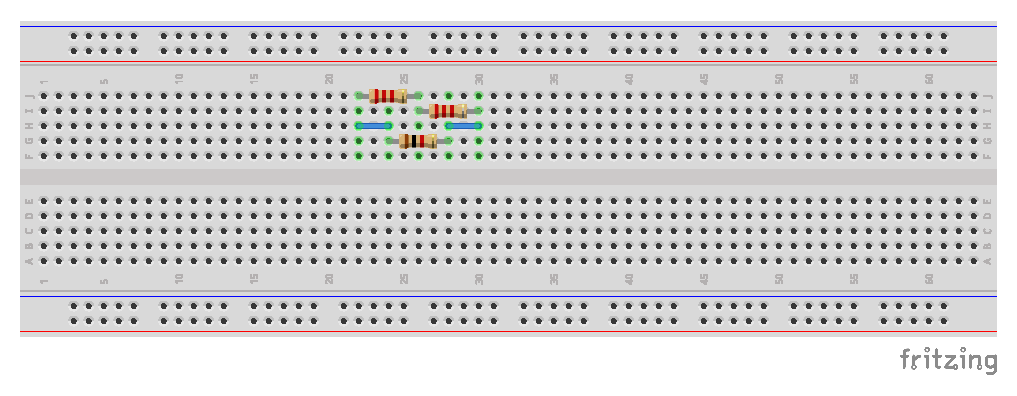
\includegraphics[scale=0.9]{a_bb.pdf}
			\caption{obwód (a)}
			\label{fig:rys3}
		\end{figure}
		\subsubsection*{Pomiar rezystancji}
		Dla obwodu z rysunku \hyperref[eq:rys2]{2} dokonano pomiaru rezystancji od strony zacisków AB przy pomocy Multimetru RIGOL skonfigurowanego do pomiaru rezystancji. Multimert wskazał wynik $808.125 \Omega$.
		
		\subsubsection*{Wyprowadzenie wzoru i obliczenie rezystancji zastępczej  dla obwodu z rysunku \hyperref[eq:rys2]{2}}
		\begin{gather*}
		R_{23}=R_{2}+R_{3}  \\
		R_{z}=\dfrac{1}{\dfrac{1}{R_{23}} + \dfrac{1}{R_{1}}} = \dfrac{(R_{2}+R_{3})R_{1}}{R_{1}+R_{2}+R_{3}}\\
		R_{z}=\dfrac{(2200\Omega+2200\Omega)1000\Omega}{1000\Omega + 2200\Omega + 2200\Omega} = \dfrac{4400000\Omega}{5400\Omega} \approx 814.8148 \Omega
		\end{gather*}
		
		\subsubsection{Obwód (b)}
		
		\begin{equation*}
		\label{eq:rys4}
		\begin{circuitikz}[scale=1,european]
		\draw
		(0,0) to [european resistor, l=$R_{1}$, a = $1k\Omega$] (0,2)
		(0,2) to (2,2)
		to [european resistor , l=$R_{3}$,a=$1k\Omega$] (5,2)
		to [european resistor, a=$ R_{5} $, l = $ 100\Omega $] (5,0)
		to [european resistor, a=$R_{4}$, l=$100\Omega$] (2,0)
		to (0,0)
		(2,2) to [european resistor, l= $2.2k\Omega$, a= $R_{2}$] (2,0)
		(2.5,-1) node[anchor = west] {A}
		to [short, o-] (2.5,0) 
		(4.5,-1) node[anchor = east] {B}
		to [short, o-] (4.5,0);
		\end{circuitikz}
		\end{equation*}
		\captionof{figure}{Obwód (b)}
		
		\subsubsection*{Budowa obwodu przy pomocy stykowej płytki prototypowej}
		Budowa obwodu przy pomocy stykowej płytki prototypowej została przedstawiona w programie Fritzing na rysunku \hyperref[fig:rys5]{5}.
		\begin{figure}[H]
			\centering
			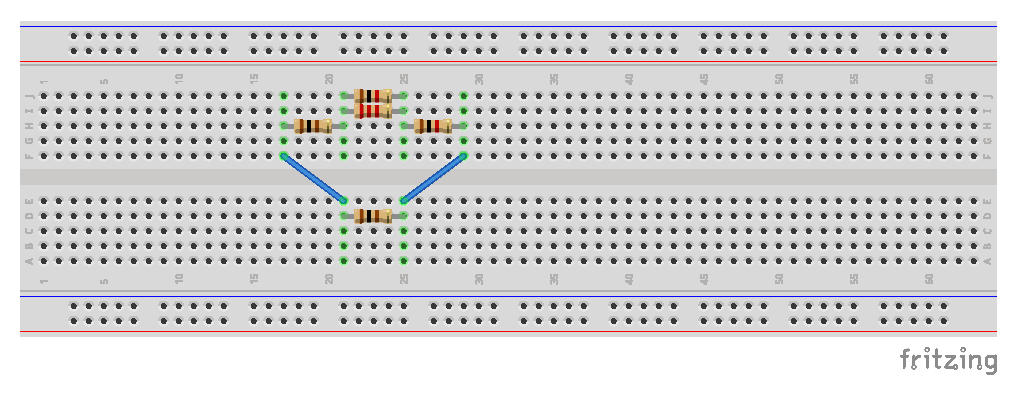
\includegraphics[scale=0.9]{b_bb.pdf}
			\caption{obwód (b)}
			\label{fig:rys5}
		\end{figure}
		\subsubsection*{Pomiar rezystancji}
		Dla obwodu z rysunku \hyperref[eq:rys4]{4} dokonano pomiaru rezystancji od strony zacisków AB przy pomocy Multimetru RIGOL skonfigurowanego do pomiaru rezystancji. Multimert wskazał wynik $95.523k \Omega$.
		
		\subsubsection*{Wyprowadzenie wzoru i obliczenie rezystancji zastępczej  dla obwodu z rysunku \hyperref[eq:rys4]{4}}
		
		\begin{gather*}
		R_{12}=\dfrac{1}{\dfrac{1}{R_{1}} + \dfrac{1}{R_{2}}} \\
		R_{1235} = R_{12} + R_{3} + R_{5} \\
		R_{z} = \dfrac{1}{\dfrac{1}{R_{4}} +  \dfrac{1}{ \dfrac{1}{\dfrac{1}{R_{1}} + \dfrac{1}{R_{2}}} + R_{3} + R_{5}}}\\
		R_{z} = \dfrac{1}{\dfrac{1}{100\Omega}} +  \dfrac{1}{ \dfrac{1}{\dfrac{1}{1000\Omega} + \dfrac{1}{2200 \Omega}} + 1000\Omega + 100\Omega} = \dfrac{14300}{151} \approx 94.7\Omega
		\end{gather*}
		
		\subsubsection{Obwód (c)}
		
		\begin{equation*}
		\label{eq:rys6}
		\begin{circuitikz}[scale=1,european]
		\draw
		(0,-0.5) node[anchor = north] {A}
		to [short, o- ] (0,0)
		(0,0) to (2,0) 
		to [european resistor, l=$R_{4}$, a=$100\Omega$] (4,0)
		to (6,0)
		(2,0) to (2,2)
		to [european resistor, l=$R_{4}$, a = $1k\Omega$] (4,2)
		to (4,0)
		(5,0) to [european resistor, a = $ R_{2} $, l = $ 2.2k\Omega $] (5,-2)
		to (6,-2)
		(1,0) to [european resistor, a= $R_{1}$, l=$2.2k\Omega$] (1,-2)
		to (0,-2)
		to [short, -o] (0,-1.5)
		(0,-1.5) node [anchor = south] {B};
		\end{circuitikz}
		\end{equation*}
		\captionof{figure}{Obwód (c)}
		
		\subsubsection*{Budowa obwodu przy pomocy stykowej płytki prototypowej}
		Budowa obwodu przy pomocy stykowej płytki prototypowej została przedstawiona w programie Fritzing na rysunku \hyperref[fig:rys7]{7}.
		\begin{figure}[H]
			\centering
			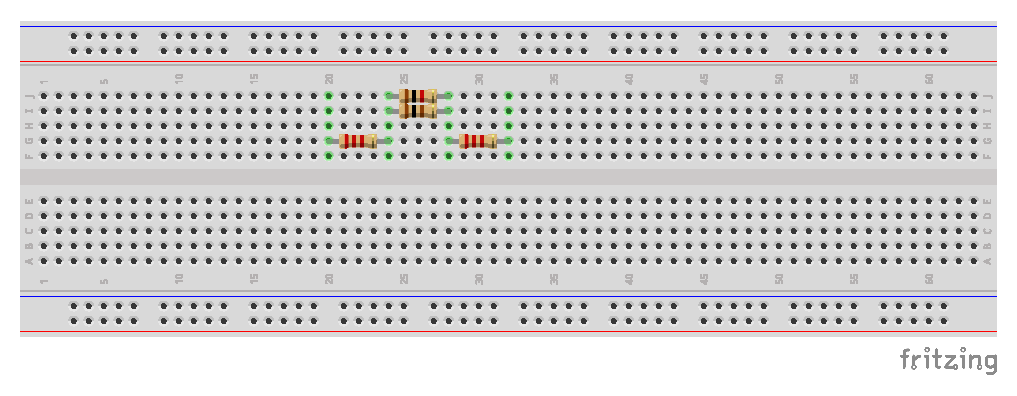
\includegraphics[scale=0.9]{c_bb.pdf}
			\caption{obwód (c)}
			\label{fig:rys7}
		\end{figure}
		\subsubsection*{Pomiar rezystancji}
		Dla obwodu z rysunku \hyperref[eq:rys6]{6} dokonano pomiaru rezystancji od strony zacisków AB przy pomocy Multimetru RIGOL skonfigurowanego do pomiaru rezystancji. Multimert wskazał wynik $2.161k\Omega$.
		
		\subsubsection*{Wyprowadzenie wzoru i obliczenie rezystancji zastępczej  dla obwodu z rysunku \hyperref[eq:rys6]{6}}	
		\begin{gather*}
		R_{z} = R_{1}\\
		R_{z} = 2200\Omega
		\end{gather*}
		
		\subsubsection{Obwód (d)}
		
		\begin{equation*}
		\label{eq:rys8}
		\begin{circuitikz}[scale=1,european]
		\draw
		(0,0) to [european resistor, l=$R_{1}$, a= $ 1k\Omega $] (2,0)
		to [european resistor, l=$ R_{2} $,a = $ 2.2k\Omega $] (5,0)
		to [european resistor, l=$ R_{5} $,a = $ 100\Omega $] (7,0)
		to (7,1)
		to (0,1)
		to (0,0)
		(2,0) to  [european resistor, a=$ R_{3} $,l=$ 2.2k\Omega $] (2,-3)
		to (6,-3)
		to [short,-o] (6,-2.5)
		(6,-2.5) node [anchor = west] {B}
		(5,-3) to [european resistor, l=$ R_{4} $, a=$ 1k\Omega $] (5,-1)
		to (5,0)
		(5,-1) to (6,-1)
		to [short,-o](6,-1.5)
		(6,-1.5) node [anchor = west] {A};
		\end{circuitikz}
		\end{equation*}
		\captionof{figure}{Obwód (d)}
		
		\subsubsection*{Budowa obwodu przy pomocy stykowej płytki prototypowej}
		Budowa obwodu przy pomocy stykowej płytki prototypowej została przedstawiona w programie Fritzing na rysunku \hyperref[fig:rys9]{9}.
		\begin{figure}[H]
			\centering
			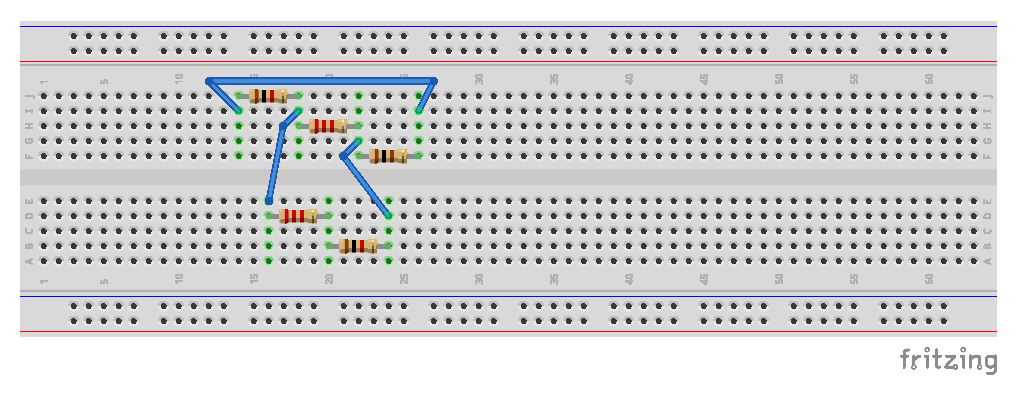
\includegraphics[scale=0.9]{d_bb.pdf}
			\caption{obwód (d)}
			\label{fig:rys9}
		\end{figure}
		\subsubsection*{Pomiar rezystancji}
		Dla obwodu z rysunku \hyperref[eq:rys8]{8} dokonano pomiaru rezystancji od strony zacisków AB przy pomocy Multimetru RIGOL skonfigurowanego do pomiaru rezystancji. Multimert wskazał wynik $739.364 \Omega$.
		
		\subsubsection*{Wyprowadzenie wzoru i obliczenie rezystancji zastępczej  dla obwodu z rysunku \hyperref[eq:rys8]{8}}	
		\begin{gather*}
		R_{51}= R_{5}+R_{1}\\
		R_{152}= \dfrac{1}{\dfrac{1}{R_{2}}+\dfrac{1}{R_{51}}}\\
		R_{3152}=R_{3} + R_{152}\\
		R_{z}= \dfrac{1}{\dfrac{1}{R_{4}}+\dfrac{1}{R_{3152}}}\\
		R_{z}= \dfrac{1}{\dfrac{1}{R_{4}} + \dfrac{1}{R_{3} + \dfrac{1}{\dfrac{1}{R_{2}} + \dfrac{1}{R_{5} + R_{1}}} }}\\
		R_{z}= \dfrac{1}{\dfrac{1}{1000\Omega} + \dfrac{1}{2200\Omega + \dfrac{1}{\dfrac{1}{2200\Omega} + \dfrac{1}{100\Omega + 1000\Omega}} }} \approx 745.76\Omega
		\end{gather*}
		
		\subsubsection{Obwód (e)}
		
		\begin{equation*}
		\label{eq:rys10}
		\begin{circuitikz}[scale=1,european]
		
		\draw
		(0,0.5) node [anchor = south] {B}
		to [short, o-] (0,0)
		to (7,0)
		(0,1.5) node [anchor = north] {A}
		to [short, o-] (0,2)
		to (3,2)
		to [european resistor, l=$R_{3}$, a= $ 2.2k\Omega $] (5,2)
		to (7,2)
		(3,2) to (3,3.5)
		to [european resistor, l =$R_{4}$, a=$ 1k\Omega $] (5,3.5)
		to (5,2)
		(2,2) to [european resistor, a=$ R_{1} $,l=$ 2.2k\Omega $] (2,0)
		(6,2) to [european resistor, a=$ R2_{2} $,l=$ 2.2k\Omega $] (6,0);
		\end{circuitikz}
		\end{equation*}
		\captionof{figure}{Obwód (e)}
		
		\subsubsection*{Budowa obwodu przy pomocy stykowej płytki prototypowej}
		Budowa obwodu przy pomocy stykowej płytki prototypowej została przedstawiona w programie Fritzing na rysunku \hyperref[fig:rys11]{11}.
		\begin{figure}[H]
			\centering
			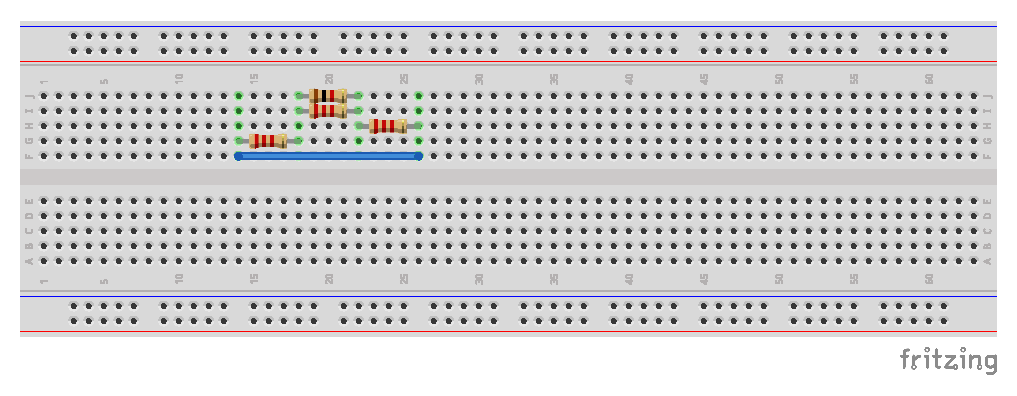
\includegraphics[scale=0.9]{e_bb.pdf}
			\caption{obwód (e)}
			\label{fig:rys11}
		\end{figure}
		\subsubsection*{Pomiar rezystancji}
		Dla obwodu z rysunku \hyperref[eq:rys10]{10} dokonano pomiaru rezystancji od strony zacisków AB przy pomocy Multimetru RIGOL skonfigurowanego do pomiaru rezystancji. Multimert wskazał wynik $1.237k\Omega$.
		
		\subsubsection*{Wyprowadzenie wzoru i obliczenie rezystancji zastępczej  dla obwodu z rysunku \hyperref[eq:rys10]{10}}	
		\begin{gather*}
		R_{34} = \dfrac{1}{\dfrac{1}{R_{3}} + \dfrac{1}{R_{4}}}\\
		R_{234} = R_{2} + R_{34}\\
		R_{z} = \dfrac{1}{\dfrac{1}{R_{1}} + \dfrac{1}{R_{234}}}\\
		R_{z} = \dfrac{1}{\dfrac{1}{R_{1}} + \dfrac{1}{R_{2} + \dfrac{1}{\dfrac{1}{R_{3}} + \dfrac{1}{R_{4}}}}}\\
		R_{z} = \dfrac{1}{\dfrac{1}{2200\Omega} + \dfrac{1}{2200\Omega + \dfrac{1}{\dfrac{1}{2200\Omega} + \dfrac{1}{1000\Omega}}}} \approx 1248.6486\Omega\\
		\end{gather*}
		
		\subsubsection{Obwód (f)}
		
		\begin{equation*}
		\label{eq:rys12}
		\begin{circuitikz}[scale=1,european]
		
		\draw
		(0,0) to (0,-2)
		to (7,-2)
		to [short, -o] (7,2.5)
		(7,2.5) node [anchor = south]	{B}
		(0,0) to [european resistor, l=$ R_{5} $, a=$ 1k\Omega $] (2,0)
		(2,-1) to (2,0)
		to [european resistor, a=$ 100\Omega $,l=$ R_{1} $] (2,2)
		to (4,2)
		to (4,1)
		to [european resistor, a=$ R_{2} $,l=$ 2.2k\Omega $] (4,-1)
		to (2,-1)
		(4,1) to [european resistor, l=$ R_{4} $,a =$ 2.2k\Omega $] (7,1)
		(3,2) to [european resistor, l=$ R_{3} $,a=$ 1k\Omega $] (3,5)
		to (7,5) 
		to [short, -o] (7,4.5)
		(7,4.5) node [anchor = north ]	{A};
		
		\end{circuitikz}
		\end{equation*}
		\captionof{figure}{Obwód (f)}
		
		
		\subsubsection*{Budowa obwodu przy pomocy stykowej płytki prototypowej}
		Budowa obwodu przy pomocy stykowej płytki prototypowej została przedstawiona w programie Fritzing na rysunku \hyperref[fig:rys13]{13}.
		\begin{figure}[H]
			\centering
			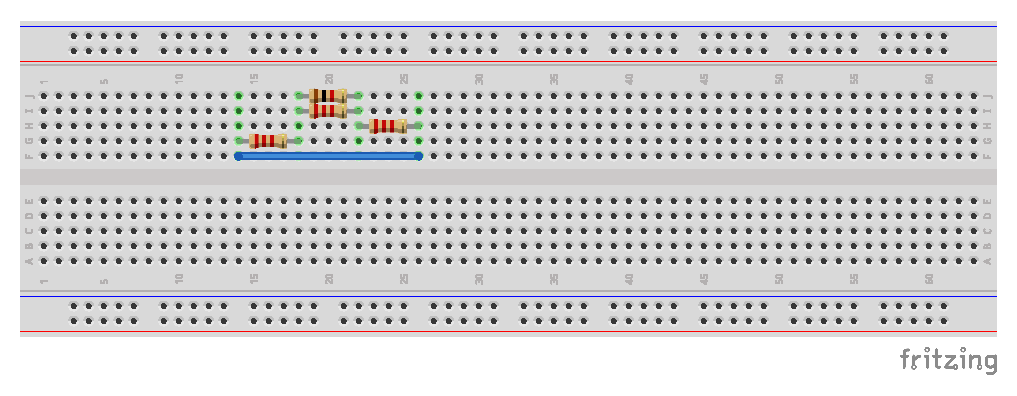
\includegraphics[scale=0.9]{e_bb.pdf}
			\caption{obwód (e)}
			\label{fig:rys13}
		\end{figure}
		\subsubsection*{Pomiar rezystancji}
		Dla obwodu z rysunku \hyperref[eq:rys12]{12} dokonano pomiaru rezystancji od strony zacisków AB przy pomocy Multimetru RIGOL skonfigurowanego do pomiaru rezystancji. Multimert wskazał wynik $1.722k\Omega$.
		
		\subsubsection*{Wyprowadzenie wzoru i obliczenie rezystancji zastępczej  dla obwodu z rysunku \hyperref[eq:rys12]{12}}	
		\begin{gather*}
		R_{12} = \dfrac{1}{\dfrac{1}{R_{1}} + \dfrac{1}{R_{2}}}\\
		R_{125} = R_{12} + R_{5}\\
		R_{1245} = \dfrac{1}{\dfrac{1}{R_{4}} + \dfrac{1}{R_{125}}}\\
		R_{z} = R_{3} + R_{1245}\\
		R_{z} = R_{3}+ \dfrac{1}{\dfrac{1}{R_{4}} + \dfrac{1}{\dfrac{1}{\dfrac{1}{R_{1}} + \dfrac{1}{R_{2}}}+ R_{5}}}\\
		R_{z} = 1000\Omega+ \dfrac{1}{\dfrac{1}{2200\Omega} + \dfrac{1}{\dfrac{1}{\dfrac{1}{100\Omega} + \dfrac{1}{2200\Omega}}+ 1000\Omega}} \approx 1731.39841
		\end{gather*}
		
		\subsubsection*{Wnioski na temat przyczyn różnic miedzy wynikami pomiarów, a obliczeń}
		
		Różnica między wynikami pomiarów, a obliczeń, może wynikać między innymi z:
		\begin{itemize}
			\item klasy dokładności przyrządów pomiarowych
			\item dokładności wykonania użytych elementów układu
		\end{itemize}
		
		
		
		\section{Pomiary napięcia}
		\subsection{Pomiar wartości napięć wyjściowych z zasilacza}
		
		\subsubsection*{Cel}
		W ćwiczeniu należy dokonać pomiaru napięcia z sekcji DC POWER SUPPLY zestawu laboratoryjnego DF
		6911, oraz odpowiedzieć na pytanie, z czego mogą wynikać ewentualne różnice między wartościami odczytanymi, a zmierzonymi.
		
		\subsubsection*{Tabela z wartościami odczytów i pomiarów}
		
		
		\[
		\begin{array}{|c|c|c|}
		\hline
		U [V]&Odczyt [V]& Pomiar [V]\\
		\hline
		1&1&1.107\\
		\hline
		3&3&3.172\\
		\hline
		4.5&4.5&4.635\\
		\hline
		11&11&11.226\\
		\hline
		13&13&13.183\\
		\hline
		25&25&25.344\\
		\hline
		28&28&28.306\\
		\hline
		\end{array}
		\]
		\captionof{table}{Wartości odczytów i pomiarów}
		
		\subsubsection*{Wnioski na temat przyczyn różnic miedzy pomiarami, a odczytami}
				Różnica między wynikami pomiarów, a odczytami, może wynikać między innymi z:
		\begin{itemize}
			\item klasy dokładności przyrządów pomiarowych
		\end{itemize}
		
		\subsection{Dzielnik napięcia}
		\subsubsection*{Cel}
		W ćwiczeniu należy, przy pomocy praw Kirchhoffa, wyprowadzić wzory oraz zależności opisujące dzielnik
		napięcia pokazany na rysunku \hyperref[eq:rysdz]{3}. Następnie należy zaprojektować dzielnik napięcia, dobierając odpowiednio rezystory i zbudować go na płycie prototypowej w taki sposób, aby na wyjściu $ V_{out} $ (spadek napięcia na rezystorze $ R_{2} $) otrzymać kolejno napięcia:
		2.5V, 3.22V, 1.66V, 4V, 4.54V. Przy realizacji każdego z dzielników należy dokonać pomiarów napięcia $ V_{out} $ i
		porównać z wartościami otrzymanymi z wyprowadzonego wzoru i dobranych rezystorów.
		\begin{equation*}
		\label{eq:rysdz}
		\begin{circuitikz}[scale=1,american]
		
		\draw
		(0,0) to[V_<=5V,i_=I] (0,4)
		to (2,4)
		to [european resistor, a=$ R_{1} $] (2,2)	
		to [european resistor, a=$ R_{2} $] (2,0)
		to (0,0)
		(2,2) to [short, -o] (3,2)
		(3,2) node [anchor = west] {+}
		(2,0) to [short, -o] (3,0)
		(3,0) node [anchor = west] {--}
		(3,1) node [anchor = west] {$V_{out}$}
		(-1,2) node [anchor = west] {$V_{in}$};
		\end{circuitikz}
		\end{equation*}
		\captionof{figure}{Rezystencjalny dzielnik napięcia}
		
		\subsubsection*{Wyprowadzenie wzoru na  $ V_{out} $ }
		\begin{gather*}
		V_{in} - IR_{1} - IR_{2} = 0\\
		IR_{2} = V_{out}\\
		I = \dfrac{V_{in}}{R_{1} + R_{2}}\\
		V_{out} = \dfrac{R_{2} V_{in}}{R_{1} + R_{2}}
		\label{eq:vout}
		\end{gather*}
		\subsubsection{Napięcie na wyjściu $V_{out} =  2.5V $}
		\subsubsection*{Projekt dzielnika napiecia w programie Fritzing}
		
		\begin{figure}[H]
			\centering
			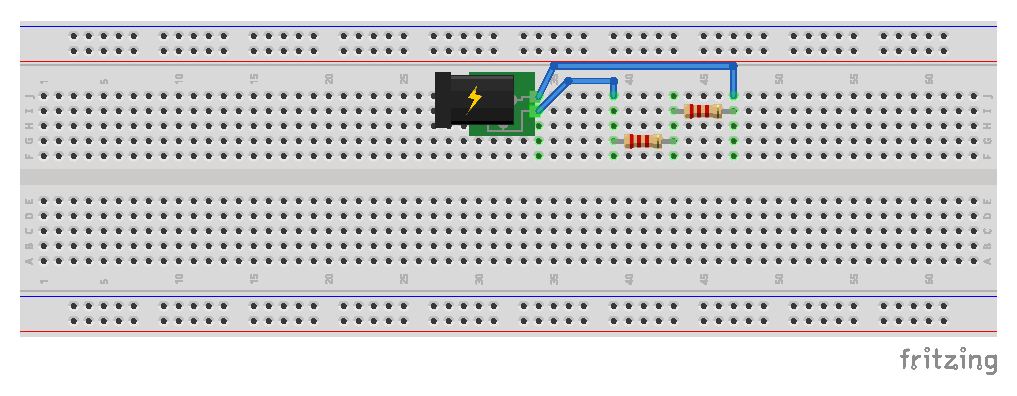
\includegraphics[scale=0.9]{2_5_bb.pdf}
			\caption{Rezystencjalny dzielnik napięcia}
			\label{fig:pod2_5}
		\end{figure}
		
		\subsubsection*{Wyznaczenie stosunku między $ R_{1} $ i $ R_{2} $ przy użyciu wyprowadzonego \hyperref[eq:vout]{wzoru}}
		\begin{gather*}
		2.5V = \dfrac{5VR_{2}}{R_{1}+R_{2}}\\
		\dfrac{2.5V}{5V} = \dfrac{R_{2}}{R_{1} + R_{2}}\\
		\frac{1}{2} = \dfrac{R_{2}}{R_{1} + R_{2}}\\
		\frac{1}{2} R_{1} + \frac{1}{2}R_{2} = R_{2}\\
		R_{1} = R_{2}\\
		\end{gather*}
		\subsubsection*{Obliczenie warości $ V_{out}$ dla rezystorów $ R_{1} = 2.2k\Omega, R_{2} =2.2k\Omega  $  przy użyciu wyprowadzonego \hyperref[eq:vout]{wzoru}}
		\begin{gather*}
		V_{out} = \dfrac{2200\Omega \cdot 5V}{2200\Omega + 2200\Omega} = 2.5V\\
		\end{gather*}
		\subsubsection*{Pomiar napięcia $ V_{out} $}
		Dla dzielnika napięcia dokonano pomiaru napięcia wyjściowego $ V_{out} $ przy pomocy Multimetru RIGOL skonfigurowanego do pomiaru napięcia. Multimert wskazał wynik $2.563V$.
		
		
		
		\subsubsection{Napięcie na wyjściu $V_{out} =  3.22V $}
		\subsubsection*{Projekt dzielnika napiecia w programie Fritzing}
		
		\begin{figure}[H]
			\centering
			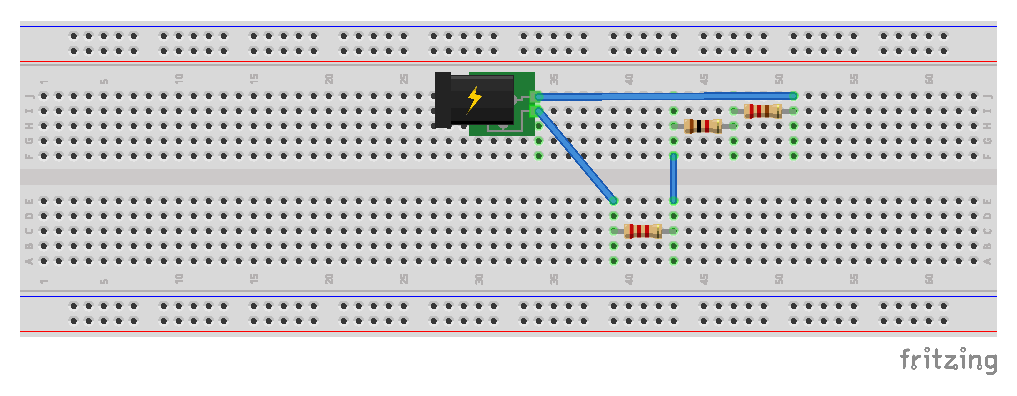
\includegraphics[scale=0.9]{3_22_bb.pdf}
			\caption{Rezystencjalny dzielnik napięcia}
			\label{fig:pod3_22}
		\end{figure}
		
		\subsubsection*{Wyznaczenie stosunku między $ R_{1} $ i $ R_{2} $ przy użyciu wyprowadzonego \hyperref[eq:vout]{wzoru}}
		\begin{gather*}
		\dfrac{3.22V}{5V} = \dfrac{R_{2}}{R_{1} + R_{2}}\\
		\frac{161}{250} R_{1} + \frac{161}{250}R_{2} = R_{2}\\
		R_{1} =\frac{89}{161} R_{2}\\
		\end{gather*}
		\subsubsection*{Obliczenie warości $ V_{out}$ dla rezystorów $ R_{1} = 1.22k\Omega, R_{2} =2.2k\Omega  $  przy użyciu wyprowadzonego \hyperref[eq:vout]{wzoru}}
		\begin{gather*}
		V_{out} = \dfrac{2200\Omega \cdot 5V}{2200\Omega + 1220\Omega} \approx 3.216V\\
		\end{gather*}
		\subsubsection*{Pomiar napięcia $ V_{out} $}
		Dla dzielnika napięcia dokonano pomiaru napięcia wyjściowego $ V_{out} $ przy pomocy Multimetru RIGOL skonfigurowanego do pomiaru napięcia. Multimert wskazał wynik $3.351V$.
		
		
		
		
		\subsubsection{Napięcie na wyjściu $V_{out} =  1.66V $}
		
		\subsubsection*{Projekt dzielnika napiecia w programie Fritzing}
		
		\begin{figure}[H]
			\centering
			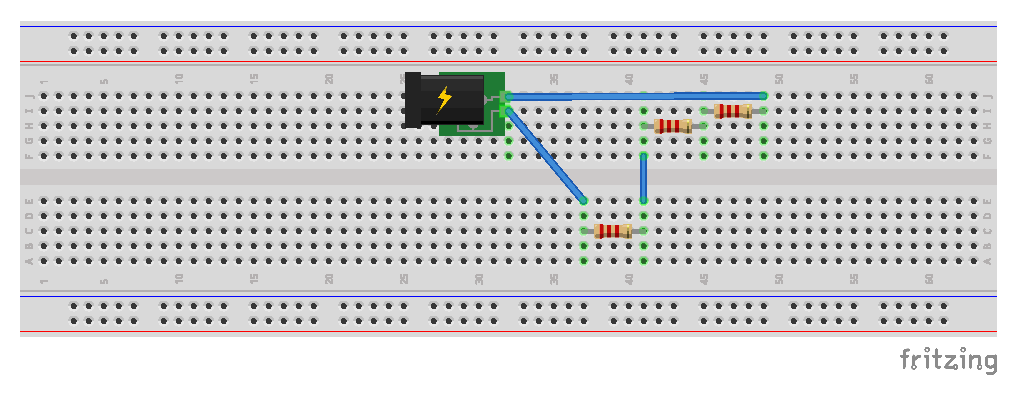
\includegraphics[scale=0.9]{1_66_bb.pdf}
			\caption{Rezystencjalny dzielnik napięcia}
			\label{fig:pod1_66}
		\end{figure}
		
		\subsubsection*{Wyznaczenie stosunku między $ R_{1} $ i $ R_{2} $ przy użyciu wyprowadzonego \hyperref[eq:vout]{wzoru}}
		\begin{gather*}
		\dfrac{1.66V}{5V} = \dfrac{R_{2}}{R_{1} + R_{2}}\\
		\frac{83}{250} R_{1} + \frac{83}{250}R_{2} = R_{2}\\
		R_{1} =\frac{167}{83} R_{2}\\
		\end{gather*}
		\subsubsection*{Obliczenie warości $ V_{out}$ dla rezystorów $ R_{1} = 4.4k\Omega, R_{2} =2.2k\Omega  $  przy użyciu wyprowadzonego \hyperref[eq:vout]{wzoru}}
		\begin{gather*}
		V_{out} = \dfrac{2200\Omega \cdot 5V}{4400\Omega + 2200\Omega} \approx 1,(6) V\\
		\end{gather*}
		\subsubsection*{Pomiar napięcia $ V_{out} $}
		Dla dzielnika napięcia dokonano pomiaru napięcia wyjściowego $ V_{out} $ przy pomocy Multimetru RIGOL skonfigurowanego do pomiaru napięcia. Multimert wskazał wynik $1.695V$.
		
		
		
		
		\subsubsection{Napięcie na wyjściu $V_{out} =  4V $}
		
		\subsubsection*{Projekt dzielnika napiecia w programie Fritzing}
		
		\begin{figure}[H]
			\centering
			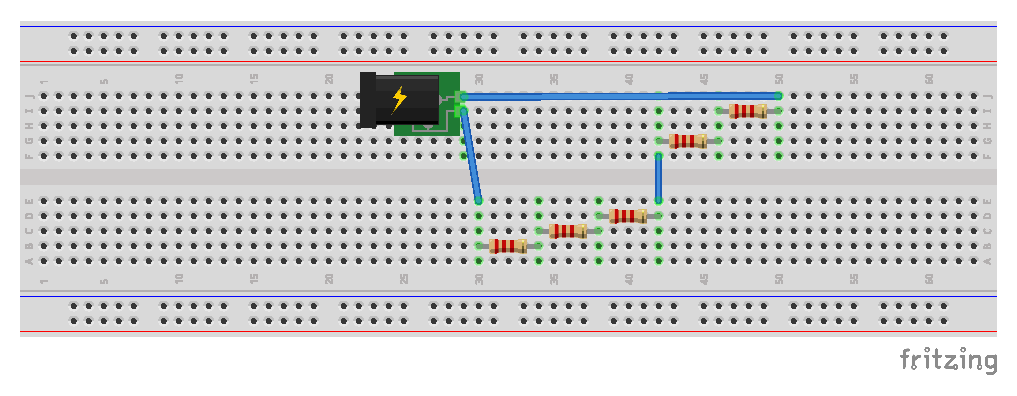
\includegraphics[scale=0.9]{4_bb.pdf}
			\caption{Rezystencjalny dzielnik napięcia}
			\label{fig:pod4}
		\end{figure}
		
		\subsubsection*{Wyznaczenie stosunku między $ R_{1} $ i $ R_{2} $ przy użyciu wyprowadzonego \hyperref[eq:vout]{wzoru}}
		\begin{gather*}
		\dfrac{4V}{5V} = \dfrac{R_{2}}{R_{1} + R_{2}}\\
		\frac{4}{5} R_{1} + \frac{4}{5}R_{2} = R_{2}\\
		R_{1} =\frac{1}{4} R_{2}\\
		\end{gather*}
		\subsubsection*{Obliczenie warości $ V_{out}$ dla rezystorów $ R_{1} = 2.2k\Omega, R_{2} =8.8k\Omega  $  przy użyciu wyprowadzonego \hyperref[eq:vout]{wzoru}}
		\begin{gather*}
		V_{out} = \dfrac{8800\Omega \cdot 5V}{8800\Omega + 2200\Omega} = 4 V\\
		\end{gather*}
		\subsubsection*{Pomiar napięcia $ V_{out} $}
		Dla dzielnika napięcia dokonano pomiaru napięcia wyjściowego $ V_{out} $ przy pomocy Multimetru RIGOL skonfigurowanego do pomiaru napięcia. Multimert wskazał wynik $4.095V$.
		
		
		\subsubsection{Napięcie na wyjściu $V_{out} =  4.54V $}
		\subsubsection*{Projekt dzielnika napiecia w programie Fritzing}
		
		\begin{figure}[H]
			\centering
			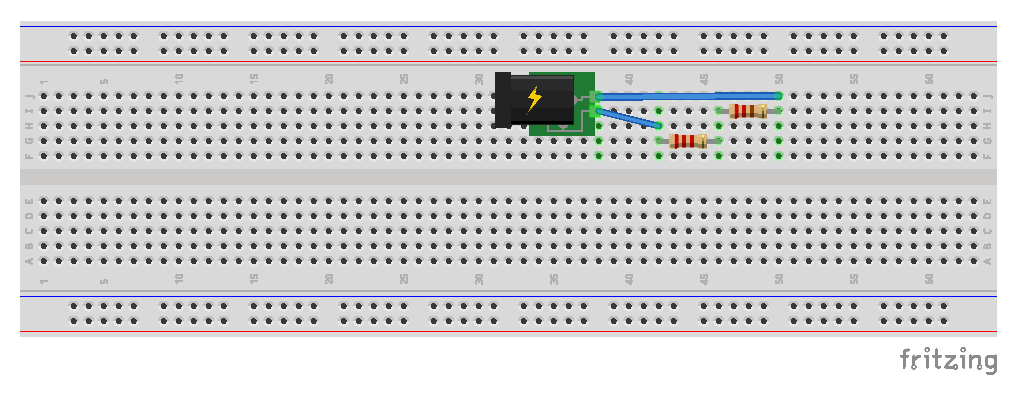
\includegraphics[scale=0.9]{4_54_bb.pdf}
			\caption{Rezystencjalny dzielnik napięcia}
			\label{fig:pod4_54}
		\end{figure}
		
		\subsubsection*{Wyznaczenie stosunku między $ R_{1} $ i $ R_{2} $ przy użyciu wyprowadzonego \hyperref[eq:vout]{wzoru}}
		\begin{gather*}
		\dfrac{4.54V}{5V} = \dfrac{R_{2}}{R_{1} + R_{2}}\\
		\frac{227}{250} R_{1} + \frac{227}{250}R_{2} = R_{2}\\
		R_{1} =\frac{23}{229} R_{2}\\
		\end{gather*}
		\subsubsection*{Obliczenie warości $ V_{out}$ dla rezystorów $ R_{1} = 220\Omega, R_{2} =2.2k\Omega  $  przy użyciu wyprowadzonego \hyperref[eq:vout]{wzoru}}
		\begin{gather*}
		V_{out} = \dfrac{2200\Omega \cdot 5V}{2200\Omega + 220\Omega} \approx 4.(54) V\\
		\end{gather*}
		\subsubsection*{Pomiar napięcia $ V_{out} $}
		Dla dzielnika napięcia dokonano pomiaru napięcia wyjściowego $ V_{out} $ przy pomocy Multimetru RIGOL skonfigurowanego do pomiaru napięcia. Multimert wskazał wynik $4.613V$.
		
				\subsubsection*{Wnioski wynikające z porównania pomiarów i obliczeń analitycznych dla sekcji 3. - Pomiary napięcia}
		
		Dokonując porównania pomiarów i obliczeń analitycznych dla sekcji 3. - Pomiary napięcia, uwzględniając błąd pomiarowy, można stwierdzić, że obliczenia i pomiary zostały wykonane prawidłowo.
		\section{Pomiary prądu stałego}
		\subsection{Pomiary prądu w obwodzie}
		\subsection*{Cel}
		Przy użyciu stykowej płytki prototypowej należy zbudować obwód pokazany na rysunku \hyperref[eq:rysob]{20} oraz dokonać pomiarów
		spadku napięcia na rezystorze R i natężenia prądu w obwodzie, pamiętając przy tym o zapisaniu jednostek.
		\begin{equation*}
		\label{eq:rysob}
		\begin{circuitikz}[scale=1,american]
		\draw
		(0,0) to[V_<=5V,i_=I] (0,2)
		to [european resistor, l=$R$, a = $2440\Omega$] (4,2) 
		to (4,0) 
		to (0,0);
		\end{circuitikz}
		\end{equation*}
		\captionof{figure}{Obwód do badania napięć i prądów }
		
		\subsection*{Wyniki pomiarów}
		
		\begin{equation*}
		\begin{array}{|c|c|}
		\hline 
		$ Natężenie prądu $&$ Spadek napięcia $\\
		\hline
		2.144 A& 5.037V\\
		\hline
		\end{array}
		\end{equation*}
		\captionof{table}{Tabela pomiarów spadku napięcia na rezystorze R i natężenia prądów w obwodzie}
		
		\subsection{Pomiary prądów i napięć}
		
		\subsection*{Cel}
		Dla obwodu z rysunków \hyperref[eq:ob2a]{21}, \hyperref[eq:ob2b]{22} należy sprawdzić prawa Kirchhoffa, dokonując stosownych pomiarów (spadki napięć na
		rezystorach oraz prądy w gałęziach) oraz obliczeń analitycznych, a następnie porównać otrzymane wartości ze
		sobą.
		
		
		
		\subsubsection{Obwód (a)}
		
		\begin{equation*}
		\label{eq:ob2a}
		\begin{circuitikz}[scale=1,american]
		\draw
		(0,0) to[V_<=5V] (0,2)
		to (2,2)
		to (2,4)
		to [european resistor, l = $ R_{4} $,a=$ 1k\Omega $] (4,4)
		to (4,2)
		to (6,2)
		(0,0) to (6,0)
		(2,0) to [european resistor, l = $ R_{1} $ , a = $ 2.2k\Omega $] (2,2)
		(4,0) to [european resistor, l = $ R_{2} $ , a = $ 2.2k\Omega $] (4,2)
		(2,2) to [european resistor, l = $ R_{3} $ , a = $ 2.2k\Omega $] (4,2)
		(-1,1) node [anchor = west] {$ V_{1} $};
		\end{circuitikz}
		\end{equation*}
		\captionof{figure}{Obwód (a) do badania prądów i napięć w obwodzie }
		
		\subsubsection*{Wyniki pomiarów}
		
		\begin{equation*}
		\begin{array}{|c|c|c|}
		\hline
		$ Rezystor $&$ Prądy w obwodzie $&$ Napięcia w obwodzie $\\
		\hline
		R_{1}&2.321mA&5.037V\\
		\hline
		R_{2}&1.763mA&4.202V\\
		\hline
		R_{3}&0.554mA&1.228V\\
		\hline
		R_{4}&1.212mA&1.573V\\
		\hline
		\end{array}
		\end{equation*}
		\captionof{table}{Tabela pomiarów spadków napięć na rezystorach oraz prądów na gałęziach}
		
				
		\subsubsection*{Obliczenia analityczne dla obwodu (\hyperref[eq:ob2a]{a})}
		
		\begin{gather*}
		R_{34} =\dfrac{1}{\dfrac{1}{R_{3}} + \dfrac{1}{R_{4}}}\\
		R_{34} = \dfrac{R_{3}R_{4}}{R_{3}+R_{4}}\\
		R_{234} = R_{2} + R_{34}\\
		R_{z} = \dfrac{1}{\dfrac{1}{R_{1}} + \dfrac{1}{R_{234}}}\\
		R_{z} = \dfrac{R_{1}R_{234}}{R_{1}+R_{234}} = 1248.65\Omega\\
		R=\dfrac{U}{I}\\
		I=\dfrac{U}{R}\\
		I=\dfrac{5V}{1248.65\Omega}\\
		I=0.004A\\
		U_{1} = 5V\\
		I_{1} = \dfrac{5V}{2200\Omega} = 0.0023A\\
		5V - I_{34}R_{34} - I_{2}R_{2} = 0\\
		I_{34} = I_{2} = I - I_{1}\\
		I_{2} = I_{34} = 0.004A - 0.0023A = 0.0017A\\
		U_{2} = I_{2}R_{2} = 0.0017A \cdot 2.2k\Omega = 3.47V\\
		U_{3} = U_{4} = U - U_{2} = 1.26V
		\end{gather*}
		
				\subsubsection*{Wnioski wynikające z porównania pomiarów i obliczeń analitycznych dla obwodu (\hyperref[eq:ob2a]{a})}
				
				Dokonując porównania pomiarów i obliczeń analitycznych dla obwodu (\hyperref[eq:ob2a]{a}), uwzględniając błąd pomiarowy, można stwierdzić, że obliczenia i pomiary zostały wykonane prawidłowo.
		
		\subsubsection{Obwód (b)}
		
		\begin{equation*}
		\label{eq:ob2b}
		\begin{circuitikz}[scale=1,american]
		\draw
		(0,0) to [european resistor, l = $ R_{2} $ , a = $ 2.2k\Omega $] (0,3)
		to [european resistor, l = $ R_{1} $ , a = $ 2.2k\Omega $] (0,6)	
		(3,6) to [V>=5V]  (0,6)
		(3,6) to [european resistor, a = $ R_{4} $, l = $2.2k\Omega$] (3,3)
		to [european resistor, a= $ R_{3} $, l= $2.2k\Omega$] (0,3)
		(3,3) to (3,0)
		to (0,0)
		(1.5,7) node [ anchor = north ] {$ V_{1} $};
		\end{circuitikz}
		\end{equation*}
		\captionof{figure}{Obwód (b) do badania prądów i napięć w obwodzie }
		
		\subsubsection*{Wyniki pomiarów}
		
		\begin{equation*}
		\begin{array}{|c|c|c|}
		\hline
		$ Rezystor $&$ Prądy w obwodzie $&$ Napięcia w obwodzie $\\
		\hline
		R_{1}&0.929mA&2.061V\\
		\hline
		R_{2}&0.464mA&1.407V\\
		\hline
		R_{3}&0.412mA&1.110V\\
		\hline
		R_{4}&0.928mA&2.290V\\
		\hline
		\end{array}
		\end{equation*}
		\captionof{table}{Tabela pomiarów spadków napięć na rezystorach oraz prądów na gałęziach}
		
				\subsubsection*{Obliczenia analityczne dla obwodu (\hyperref[eq:ob2b]{b})}
		
		\begin{gather*}
		R_{23} = \dfrac{1}{\dfrac{1}{R_{2}} + \dfrac{1}{R_{3}}}\\
		R_{23} = \dfrac{R_{2}R_{3}}{R_{2}+R_{3}}\\
		R_{z} = R_{4} + R_{1} + R_{23}\\
		R_{z} = R_{4} + R_{1} + \dfrac{R_{2}R_{3}}{R_{2}+R_{3}}\\
		R_{z} = 4400\Omega + \dfrac{4840000\Omega}{4400\Omega}	 = 5500\Omega\\
		R_{z} = \dfrac{U}{I}	\\
		I = \dfrac{U}{R_{z}}\\
		I = \dfrac{5V}{5500\Omega} = 0,0009A\\
		R = \dfrac{U}{I}\\
		U = IR\\
		U_{1} = I_{1}R_{1}\\
		I_{1} = I_{4}\\
		R_{1} = R_{4}\\
		U_{1} = U_{4}
		U_{1} = 0.009A \cdot 2200\Omega\\
		U_{1} = 1.98V\\
		U_{4} = 1.98V\\
		R_{2} = R_{3}\\
		I_{2} = I_{3}\\
		I_{2} = \frac{1}{2}I_{1}\\
		I_{2} = 0.00045A\\
		U_{2} = 0.00045A \cdot 2200\Omega = 0.99V\\
		U_{3} = 0.99V
		\end{gather*}
		
		\subsubsection*{Wnioski wynikające z porównania pomiarów i obliczeń analitycznych dla obwodu (\hyperref[eq:ob2b]{b})}
		
						Dokonując porównania pomiarów i obliczeń analitycznych dla obwodu (\hyperref[eq:ob2b]{b}), uwzględniając błąd pomiarowy, można stwierdzić, że obliczenia i pomiary zostały wykonane prawidłowo.
		
		\newpage
		
		\tableofcontents
		
	\end{spacing}
\end{document}


